\documentclass[notitlepage,12pt]{article}

% Packages to use
\usepackage{setspace}
\usepackage[table]{xcolor}
\usepackage{booktabs}
\usepackage{booktabs}
\usepackage{longtable}
\usepackage{lipsum}
\usepackage{graphicx}
\usepackage{natbib}
\usepackage[margin=1in]{geometry}
\usepackage{fancyhdr}
\pagestyle{fancy}
\usepackage{float}
\rhead{S. Hogan-H}
\lhead{Which Trend in Intergenerational Income Mobility?}
\usepackage{setspace}
\doublespacing
\usepackage[flushleft]{threeparttable}
\usepackage{longtable}

\usepackage[english]{isodate}
\usepackage{hyperref}
\usepackage{amsmath}

% Author
\author{Senan Hogan-H\footnote{Undergraduate Research and Teaching Assistant at the Department of Economics, Pomona College. \newline This research was funded by the Pomona College Summer Undergraduate Research Project Fund, and I am very grateful for the help and supervision provided by the programme and Michael Steinberger, Pomona College.}}

% Title
\title{
Which Trend in Intergenerational Income Mobility? \\ \large{Regression-Based Measures of Intergenerational Income Mobility in the Panel Study of Income Dynamics (PSID)}}



\date{29 August 2017  \\
\vspace{15mm}
\textit{Working Paper}\footnote{\href{https://drive.google.com/file/d/0BwswqzI6_NHTdlFaM29Za3JnS0E/view?usp=sharing}{\color{blue}{\underline{A summary of this paper is available in poster form, in accordance with SURP funding requirements.}}}}}


%%% BEGIN %%%
\begin{document}
\maketitle
\thispagestyle{empty}
% Abstract
\begin{abstract}
I present evidence on static  estimates and time trends in intergenerational income mobility for the US using survey data by the dominant regression-based measures: the intergenerational elasticity of income and intergenerational rank-rank association.  I find the intergenerational income elasticity and rank-rank association to be estimated around 0.4 and 0.3 respectively, and evidence regarding changes across the income distribution and across demographic groups to be less conclusive.  A negative trend is found by both measures 1980--2014, in contrast to previous studies.  Lastly, I consider what these results mean for studies that attempt to show trends in mobility in our dynamic and changing economy, with application to between group comparisons and using survey data in the study of intergenerational mobility.
\end{abstract}

\newpage
\setcounter{page}{1}

% Introduction
\section{Introduction}

There is a growing perception that intergenerational mobility is falling in the US.  The fall in mobility is often given in the broader context of rapidly rising income and wealth inequality, zoning restrictions and de facto segregation by income and race, or even advantages for the wealthy in the tax code and the colleges admissions process.\footnote{See \cite{reeves2017dream} for a non-technical overview and discussion of these issues.}  The economic literature has focused largely on estimating static measures intergenerational income mobility, and recently has been mixed on finding a time trend for recent years.

I present regression-based measures for intergenerational income mobility, and apply them to Panel Study of Income Dynamics (PSID) in order to build on the work and methods of \cite{lee2009trends} and \cite{chetty2014united}.  I also apply the methods in various methods for differences in intergenerational mobility to demonstrate what lacks in the regression-based measures, especially when applied to (limited) survey data.  I go on to discuss the use of non-parametric measures in comparison.

I estimate intergenerational income mobility for representative survey participants born between 1950 and 1989, and time trends observed over 1977--2014.  The measures considered are the intergenerational income elasticity and the intergenerational rank-rank association.  I find that the measures show a small but significant downward trend in mobility over time, wild deviations in mobility across groups (by interaction-based regressions methods), and unstable trends when estimated across quantiles.  These findings shine new light on trends in intergenerational mobility, updated to newer data for 2014, and demonstrate how traditional regression-based measures of intergenerational mobility perform in studies applied to limited survey data. 

My paper is structured as follows.  Section 2 surveys current literature on intergenerational income mobility.  Section 3 describes a framework for measuring intergenerational income mobility in multiple different ways with empirical specifications, as well as a description of the PSID data set they are applied to.  Section 4 presents the empirical results of each measure.  Section 5 discusses the findings of the paper, with lessons to learn for studies that use larger, more reliable administrative data sets in studying intergenerational income mobility.

% LIT REVIEW
\section{Literature Review}
The idea of the American Dream was popularised in \cite{truslow1938epic}, and was dependent on the idea of equality of opportunity: ``Opportunity for each according to ability or achievement," and not opportunity according to social status and birth as in the (then) old world.  It follows that a level of intergenerational mobility, relative change in status or social ranking across generations, plays important part in maintaining the American Dream.\footnote{While research on mobility is regularly discussed in the context of inequality of opportunity (as they should be), direct applications to opportunity are not directly straightforward -- i.e. stability in intergenerational mobility may not directly imply stability regarding equality of opportunity, as often stated.  See \cite{van2001three} for a rigorous structure on this interconnection.}  Income is the main measure for social status used in intergenerational mobility studies, so that previous research has concentrated on the statistical and econometric relationship between the income of children and their parents.  However, there is not universal agreement on the measurement of intergenerational income mobility.

\cite{solon1992intergenerational} popularised the use of the intergenerational income elasticity (IGE -- see section 3.1) to measure intergenerational income mobility.  Longitudinal panel data that are linked to parents and representative for the US population are relatively inabundant so that \cite{solon1992intergenerational} was the first to study mobility using such a data set (PSID), estimating the IGE to be at least 0.4.\footnote{Whereas previous IGE estimates were biased downward by using data samples with significant measurement error and/or unrepresentative samples.}  Furthermore, \cite{lee2009trends} adjusted the methods to estimate time trends in the IGE, estimating the IGE around 0.4 to 0.5 and not declining from 1977--2000.

More recently, other statistical measures for mobility have become more common.  \cite{chetty2014united} argue that a rank-rank association is a better measure of intergenerational mobility as it only depends on the joint distribution of parent and children's incomes.  They apply this method to IRS administrative data to find no fall in mobility for cohorts born between 1971 and 1993.  \cite{chetty2014land} use similar methods to find vast differences in mobility according to locality in the US, as well as the characteristics of localities associated with high or low in mobility.

Transition probabilities, often presented as part of matrices, have been especially useful to show differences in mobility according to demographics.  
\cite{shorrocks1978measurement} defined a transition matrix as rows of corresponding probabilities for movement from defined positions to another defined position (regularly quantiles) in the income distribution.  \cite{Mazumder2014} does note the persistent lower mobility for African-Americans by this measure, contending that there are surprisingly few studies that specifically focus on probabilities of reaching a top income quantile for children born to lower quantile parents, and racial demographics.\footnote{Especially given how conditional probabilities lend to splitting probabilities by demographic differences.}  However, transition matrices are regularly used as a centre-point in reports, such as \cite{blanden2005intergenerational} and \cite{sawhill2008trends}, due to their non-technical nature and ease of understanding.  \cite{chetty2014united} see no change in probability of children born to parents in the bottom quintile of income reaching the top for cohorts born between 1971 and 1993.

\cite{bhattacharya2011nonparametric} develop a newer measure for intergenerational mobility to consider differences between white and black Americans, with National Longitudinal Survey of Youth data. They find that black Americans experience lower relative upward mobility than white Americans, and that lower adolescent  cognitive skills (as measured by test scores) largely explain the difference.  \cite{chetty2017fading} explore absolute upward mobility in the US with administrative data to show a massive decline for cohorts born between 1940 and 1984, related to a change in the distribution of gain from economic growth over the corresponding time period.

Over the same time that previous studies have looked at intergenerational mobility, there are notable dynamics at play in the US economy at large.  Geographic mobility, by interstate interstate migration, has decreased steadily since the 1980s according to \cite{NBERw20065}.  A racial income gap persists in the 21st century -- see \cite{reich2017racial} for an overview of research on racial income disparities.  And there has been a pronounced increase in income inequality over the second half of the 20th century, illuminated in the world famous ``Capital in the 21st Century'' by \cite{piketty2017capital}.  

There are a few studies that have examined how demographics and wider dynamics affect intergenerational income mobility.  \cite{corak2013income} compares mobility across developed nations (by the IGE) with a view to show differences in public policy, inequality and mobility.  \cite{krueger2012rise} famously took Corak's ideas further by presenting the ``Great Gatsby Curve,'' where higher inequality is negatively correlated with social mobility and implied to cause lower mobility.  \cite{eide1999factors} use quantile regression to show a static lower mobility (by the IGE) for poorer quantiles, mainly explained by differences in education.  Lastly, \cite{nichols2009detailed} are critical of regression and probabilistic based approaches to measuring mobility, instead focusing on the median and 10th, 90th percentiles to get a picture of mobility obscured by common measures.

This paper uses the mentioned regression-based measures of intergenerational income mobility, applied to a widely used longitudinal data set.  The results are presented in the wider context of lessons learned from the mentioned studies to demonstrate some problems that studies using traditional regression-based measure and survey data to examine intergenerational mobility run in to.

% Methods
\section{Methods and Empirical Specifications}
The Panel Study of Income Dynamics is the longest running longitudinal household survey in the world.  It collects information on individuals by survey biennially for 18,000 individuals living in 5,000 families in the US, and provide sample weights to be used to represent the population of the US.  The Survey ran annually from 1968 to 1997 and biannually since -- up to most the most recent information available for 2015 (income for 2014).  Most importantly, PSID provides \textit{The Family Identification Mapping System}, a tool used to match individuals with their parents and thus generate a sample including variables for both children and their matched parents.  This makes the PSID a great resource for intergenerational income research, to analytically compare the income of individuals to the income of their parents.  It should be noted, too, that the PSID collects information mainly at the household and family level, for example by reporting household income as opposed to income per individual.  It follows that analysis pertaining to income in the PSID regularly use family level data, as will this analysis.

\begin{figure}[H]
  \centering
  \caption{Income by group comparisons and year observed.}
  \includegraphics[width=6.5in]{Graph20.pdf}
\end{figure}

Figure 1 shows average family income among the comparisons groups each year 1977--2014.  The income measure is a long-run income measure described in section 3.1.  The immobile group, where household heads live in the same area they grew up in, have an income persistently lower than the mobile group, but the differences are not pronounced.  On the other hand, households with a black head have significant and persistent lower average income than those with white heads.  As such, the comparisons for mobility are devised to be comparisons first between groups with no significant difference in average income (mobile vs immobile), then a comparison for groups with a significant difference in average income (black vs white).

\subsection{Intergenerational Income Elasticity (IGE)}

The IGE is the most commonly used measure for intergenerational income mobility, and is defined as follows.

Let $Y$ and $X$ be the log function for measures of long run income for children and parents respectively.\footnote{Only counting positive, non-zero incomes for continuity.}  Then the IGE is defined as the coefficient $\beta$ to be estimated in the least squares regression model (1), where $\alpha$ denotes a constant term and $\varepsilon$ the error term.
\begin{equation}
Y=\alpha + \beta X + \varepsilon
\end{equation}
Let $\sigma_Y$ and $\sigma_X$ be the respective standard deviations for $Y$ and $X$, so that the IGE is given in equation (2).
\begin{equation}
\beta = \frac{\textnormal{Cov} [Y, X]}{\sigma_Y \sigma_X}
\end{equation}
$\beta$ is interpreted as a measure of intergenerational income mobility as estimating $\beta=1$ implies that the income of children is perfectly associated with income of their parents, and so perfect immobility.  Conversely, estimating $\beta=0$ implies that there is no predictive relationship between income of children and parents, and so perfect mobility.  \cite{black2010recent} note how the IGE depends on the marginal distributions of income for both children and parents as well as the joint distribution between them.\footnote{This point is expanded on in section 3.2.}  The exact regression model can be adjusted for purpose, such as including interaction terms for relevant dummy variables or a function of controls, without compromising interpretation of the IGE estimated coefficient.

I estimate the last squares model (1) in multiple ways, separately for children born in 1950--1959, 1960--1969, 1970--1979 and 1980--1989.  The income measure for children is income for their family unit averaged between ages 28--30 in 2012 dollars by the CPI-U, and for parents family income averaged over the years where their children are 15--17.\footnote{The parent family income is averaged between family income of the child's father and mother.  For the vast majority of children, mother and father live in the same household and thus have the same family income, so that the average is equal to either parent's income in the majority and averaged across both parent's income when they are not.  When only one parent's income is available, it is taken as that parents income.}  Negative and zero incomes are excluded, as are incomes above \$10,000,000.\footnote{The PSID recommends that extreme outliers are excluded in this manner.}  These conditions for inflation adjustment and excluding outliers are used throughout section 3. 

First I apply ordinary least squares to the model for a standard IGE.  Secondly, I estimate various quantile regressions for estimates of the IGE by different quantiles.  Thirdly, I take an interaction-based approach to estimate the IGE by race and geographic mobility.  I estimated the same model, with dummy variables interacted with parental income in order to show estimated IGE for household with a head-of-household who is black, and separately I estimate the same model with dummy variable with interactions for the head of household the children live in resides in the same state they grew up in (for years income taken).  It follows that the IGE can be compared by the above manners across the income distribution, for black headed and the white headed families, and for households headed by people who live in the same state they grew up in to compare for geographic mobility.

Next, I use the \cite{lee2009trends} approach to show trends in the IGE observed for 1977--2014, in regression model (3).  This model uses every year of income reported in the PSID to more efficiently use available observations, while controlling for age of the children for each income observation.
\begin{multline}
Y_{ict}=\alpha'D_t
+ \beta_t X_{ic} 
+ \gamma_1 A_{ic}  
+ \gamma_2 A_{ic}^2
+ \gamma_3 A_{ic}^3 
+ \gamma_4 A_{ic}^4
+ \delta_1 (t-c-40)
+ \delta_2 (t-c-40)^2
+ \delta_3 (t-c-40)^3  \\  
+ \delta_4 (t-c-40)^4
+ \theta_1 X_{ic} (t-c-40)
+ \theta_2 X_{ic} (t-c-40)^2
+ \theta_3 X_{ic} (t-c-40)^3
+ \theta_4 X_{ic} (t-c-40)^4
+ \varepsilon_{ict}
\end{multline} 
Here, $Y_{ict}$ denotes the log function of children family income observation $i$, observed in year $t$, part of cohort (i.e. born in year) $c$.  $\alpha_t$ is the fixed effect for each year, combined with $D_t$ vector with dummy variable for year $t$.  $X_{ic}$ is the log function of family income for the children's parents\footnote{Matched as before, described in footnote 7.} averaged over the years when the children were 15--17; $A_{ic}$ is the age of the parent's head of household when parental income is observed;  $(t-c-40)$ is the age of the child (when the children income is observed) minus 40.  So that the regression controls for a quartic in parental age, in child’s age, and interactions of the child’s age quartic with parental income.  Children income observation are considered in a pass through approach where children those age 25 are considered in the 1977 (cohort 1952) regression, those aged between 25 and 26 in 1978  (cohorts 1952, 1951), and continued for those aged between 25 and 62 (cohorts 1951--1989) in 2014.\footnote{\cite{lee2009trends} present the full reasoning for the to time trends in the IGE.}  The children age variable is normalized to equal 0 at age 40, in order to  simplify interpretation of the $\beta_t$ vector as the IGE at child’s age 40 evolves as cohorts pass through that age.\footnote{\cite{lee2009trends} reference \cite{Haider2007} and \cite{bohlmark2006life} in that errors-in-variables bias for left-hand side variable mismeasurement error is minimised if taken as measured at age 40.}$^,$\footnote{The choice to show trends in the IGE for an observed time trend as opposed to by trends by year of birth cohort is noted as an arbitrary choice by \cite{lee2009trends}.}  

Ordinary least squares is applied to regression model (3) to show general trend in the IGE over 1977--2014.\footnote{Quantile regressions and interactions are non-stable for trends using the PISD, can bee seen in the Appendix.}  I use robust standard errors clustered around individuals -- as by \cite{lee2009trends}  -- in order to control for heteroskedacity and observations of repeated individuals/families between time periods.

\subsection{Intergenerational Rank Association (IRA)}
The IRA is an updated regression-based version of measure intergenerational mobility, and is defined as follows.

The income for children and parents are ranked relative to to their respective others in the distribution.  Let $U$ and $V$ be the resulting distribution of ranks for children and parents.  Then the rank-rank association is defined as the coefficient $\rho$ in the least squares model (4), where $\eta$ denotes the constant term to be estimated and $\varepsilon$ the error term.

\begin{equation}
U=\eta + \rho V + \varepsilon
\end{equation}

$\rho$ is to be interpreted in a similar way to the IGE for intergenerational mobility, but for a predictive nature between the relative rank of the parents in the income distribution for the rank of their children.  \cite{dahl2008association} first used the IRA to build on earlier work that mainly used the IGE, showing that the IRA is shows less bias (or variation) in estimates according to age at which income is measured, for either children or parents, than the IGE.  \cite{chetty2014land} build on this work further by demonstrating how the IRA only depends on the joint distribution of income for parents and children, and is thus a better measure of mobility.\footnote{In contrast, the IGE depends on both marginal distributions of income for parents and children, as well as the joint distribution.  It follows that trends over time in the IGE contend with differences in the marginal distributions as compare to each other, such as a rise in variance in income (say, for growing income inequality) for the children's distribution, but not for the parents' (measured a number of years earlier) compared to previous estimates.  So that estimates in the IGE have questions regarding their comparability across different time periods.}

I estimate the last squares model (1) in multiple ways, separately for children born in 1950--1959, 1960--1969, 1970--1979 and 1980--1989.  First I apply ordinary least squares to the model for a standard IRA estimate.  Secondly, I estimate various quantile regressions for estimates of the IRA by different quantiles.  Thirdly, I take an interaction-based approach to estimate the IGE by race and geographic mobility.  These methods are directly comparable to the those in section 3.1, adjusted to estimate the IRA.  Children's income at ages 28--30 is ranked relative to others in the same birth cohort, while their parent's income for the year's when their children are 15--17 is also ranked relative to others in the same birth cohort (for their children).  As by \cite{chetty2014united}, I divide parent income ranks into 50 to reduce noise.

Next, I adjust the approach in section 3.1, and by \cite{lee2009trends}, to show time trends in the IRA, in regression model (5).  Once again, this approach uses the available data in the PSID more efficiently, while also controlling for age in years income rank is observed.

\begin{multline}
U_{ict}=\eta'D_t
+ \rho_t V_{ic} 
+ \gamma_1 A_{ic}  
+ \gamma_2 A_{ic}^2
+ \gamma_3 A_{ic}^3 
+ \gamma_4 A_{ic}^4
+ \delta_1 (t-c-40)
+ \delta_2 (t-c-40)^2
+ \delta_3 (t-c-40)^3  \\  
+ \delta_4 (t-c-40)^4
+ \theta_1 V_{ic} (t-c-40)
+ \theta_2 V_{ic} (t-c-40)^2
+ \theta_3 V_{ic} (t-c-40)^3
+ \theta_4 V_{ic} (t-c-40)^4
+ \varepsilon_{ict}
\end{multline} 

Here, $U_{ict}$ denotes the rank of children family income observation $i$, observed in year $t$, part of cohort (i.e. born in year) $c$.  $\eta_t$ is the fixed effect for each year, combined with $D_t$ vector with dummy variable for year $t$.  $V_{ic}$ is the rank of family income for the children's parents averaged over the years when the children were 15--17; $A_{ic}$ is the age of the parent's head of household when parental income is observed;  $(t-c-40)$ is the age of the child (when the children income is observed) minus 40.  

The children ranks are constructed by order income for each (available) year of birth separately, including every year of income observed.  The parent ranks are also constructed according to the year of birth of their children, and (as described) instead include a long-run measure for income.  The same passing through sample restriction applies as in section 3.1, as does interpretation of the $\rho_t$ vector as IRA at child's age of 40 changes as subsequent cohorts pass through that age.  Ordinary least squares is applied to regression model (5).\footnote{Quantile regressions and interactions are non-stable for trends using the PISD, can bee seen in the Appendix.}

% RESULTS
\section{Results}
Results for this study are presented in sections 4.1 and 4.2 as graphical representations of the relevant estimated coefficients for ease of comparison, see Appendix I for presented tables with summary statistics. 

\subsection{Intergenerational Income Elasticity (IGE)}
\begin{figure}[H]
  \centering
  \caption{IGE Estimates by Decade of Birth}
  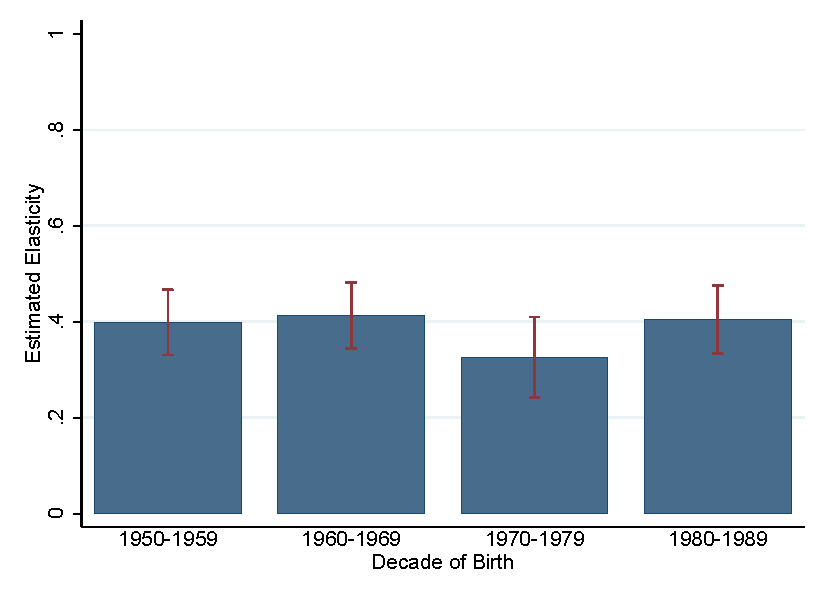
\includegraphics[width=4in]{Graph1.pdf}
\end{figure}
Figure 2 shows my general estimates of the IGE for cohorts born in four sequential decades, with error bars representing the 95\% confidence intervals.  The results are grouped around 0.4, and none statistically significantly different from each other at any reasonable level of confidence (by Wald test analysis).  IGE estimates of around 0.4\footnote{Or slightly above within the given confidence intervals.} are consistent with the vast majority of studies that predict the IGE with long-run measures of income both children and their parents, including by \cite{solon1999intergenerational} measuring the IGE for the US in the 1990s.  The confidence intervals also by majority contain higher static predictions of the IGE, which range between 0.4 and 0.5 by \cite{solon1992intergenerational} and \cite{zimmerman1992regression}.  Children born in the 1970s have a predicted IGE of 0.33, lower than the IGE estimated IGE for the other three decades of birth, which are practically equal at 0.4.  These results imply that the IGE has no statistically significant differences when compared across people born across these four decades.
\begin{figure}
  \centering
  \caption{IGE Estimates by Quantile Regression and Decade of Birth}
  \includegraphics[width=4in]{Graph22.pdf}
\end{figure}

Figure 3 show my estimates for the IGE in the same manner as Figure 2, but compared for nine sequential quantile regressions (as labelled).  Children born in the 1950s see the largest differences in the IGE by quantile, with quantiles 0.1 and 0.2 exhibiting significantly higher estimates in the IGE than any other quantile, 0.59 for quantile 0.1 and 0.47 for quantile 0.2.  Quantiles 0.5 through 0.9 exhibit an estimated IGE lower than that for the ordinary least squares estimate.  This would imply that the bottom of the income distribution experiences lower mobility than the rest of the income distribution (by this measure) and higher mobility for those further up the income distribution, but the same results do not hold for all the other decades of birth.

Children born in the 1960s see a higher IGE estimate for the 0.1 quantile of 0.5, but this result is not significantly different from estimates for quantiles 0.2 through 0.5.  The top 5 quantiles exhibit largely similar estimates of the IGE, slightly lower than 0.4.  Children born in 1970s again have the highest IGE estimate for the 0.1 quantile of 0.47, not as high as estimated for the 1950s.  The next quantiles show a ``u-shape" in the IGE, where the lowest estimates are for the middle quantile 0.5 of 0.27.  Lastly, children born in the 1980s show no significant differences in the IGE for any quantile, showing an estimated IGE of around the same ordinary least squares estimate for all quantiles.\footnote{As mentioned in section 5, the regressions for the 1980s have the lowest number of observations, making for results greater confidence intervals and more problems in comparison than the other decades.}

\begin{figure}
\centering
\begin{minipage}{.47\textwidth}
  \centering
  \caption{IGE Estimates by Interaction Terms for Race.}
  \includegraphics[width=\textwidth]{Graph3.pdf}
  \end{minipage}
\begin{minipage}{.47\textwidth}
  \centering
  \caption{IGE Estimates by Interaction Terms for Geographic Mobility.}
  \includegraphics[width=\textwidth]{Graph4.pdf}
  \end{minipage}
\end{figure}
Figure 4 shows estimated IGE for households with white heads compared to households with black heads, by interaction with the relevant dummy variable.  Children in households with a black head have estimates of the IGE higher than those in households with white heads for those born in the 1950s, 1960s and 1980s.  They exhibit a much lower IGE in the 1970s,\footnote{The decade of birth 1970s is noted as having the lowest number of black individuals surveyed by the PSID in all comparing decades.} where the 95\% confidence interval is below 0 (not shown in Figure 3).  However, none of these differences are significant by Wald test comparisons. 

Figure 5 shows results for a very similar interaction based approach to Figure 3, but instead comparing children part of households when the head grew up in the same state and region in which they now live (immobile) and children who are part of households where the head lives in a separate region and state (mobile).  None of the results are significantly different between the groups, with estimates around 0.4, though children in the 1980s part of an immobile households exhibit an IGE of 0.45, 0.13 points higher than their mobile counterparts.  Figures 3 and 4 exhibits the unfortunate inability of showing intergenerational mobility by the traditional IGE regression based measured – as discussed in section 5.

\begin{figure}
  \centering
  \caption{Estimated IGE by Year.}
  \includegraphics[width=6in]{Graph5.pdf}
\end{figure}
Figure 6 presents the consecutive results for IGE estimates in equation (3), with 95\% confidence intervals given by the dashed lines, for the years observed 1980--2014, extending the methods and results by \cite{lee2009trends} fourteen years.\footnote{Though the estimates are not split according to gender in my results.}  The results are normalised for an elasticity for 40 year olds in each year.   IGE estimates for 1977--1979 are not shown as they are not found to be statistically significantly different from zero for each of those years, as a result of the pass through process of sample selection where the earlier years uses small samples and so give less precise estimates than do the following years.  

The year 1980 has an associated IGE estimate of 0.22, before rising in the next four years to 0.45 in 1984.  Such a drastic rise in the IGE is not to be expected over such a short time period, and is presumably a results of only younger cohorts being included for the consecutive years 1980--1983, as described by \cite{lee2009trends} for daughters in their specification.  After 1983, the IGE estimate stabilises around 0.47, before dropping to 0.41 in 1998.  Subsequently the IGE estimates rise to 0.54 in 2008, and stay about the same for an estimate of 0.52 in 2014.  The average of the 25 (statistically significant) yearly estimates\footnote{Where later years are double weighted for completeness.}  is 0.47, a fairly typical estimate relative to the relevant literature surveyed by \cite{solon1992intergenerational}, and where no (significant) yearly estimate beyond 1982 differs from by more than 0.1.

Wald tests for equality and OLS regression for time over the years 1977--2000 find no significant decrease in mobility, so replicating the same result for \cite{lee2009trends}.  However, running an OLS regression for time 1980--2014 yields a positive coefficient of 0.004 (0.001), significant at the 1\% level.  The same test for 1984--2014 finds a coefficient of 0.002, significant only at the 10\% level of confidence.  These results would imply different conclusions about time trends in mobility by the IGE, which are addressed in section 5.  Lastly, quantile regressions and interaction based for this approach do not exhibit stability in estimates for the IGE, and are presented in Appendix II.

\subsection{Intergenerational Rank Association (IRA)}
\begin{figure}[H]
  \centering
  \caption{IRA Estimates by Decade of Birth}
  \includegraphics[width=3in]{Graph9.pdf}
\end{figure}
Figure 7 presents IRA estimates by decade of birth, with error bars for the 95\% confidence intervals.  All estimates lie between 0.3 and 0.4, with the 1970s cohorts exhibiting the lowest IRA of 0.31 and the 1980s highest of 0.39.  None are significantly different from any of the others (by Wald test for equality).  The results are similar to estimates for the IGE, similar but around 0.01 to 0.05 points lower.  In this manner, the IGE and IRA comparisons are very similar to differences found by \cite{dahl2008association}.  The confidence intervals are each near 0.43, and bounded below by varying figures between 0.24 and 0.33.  These results imply no significant differences in mobility as measured by the IRA across these four decades of birth.  
\begin{figure}[H]
  \centering
  \caption{Graphical Representation of the IRA.}
  \includegraphics[width=4in]{Graph16.pdf}
\end{figure}

These results find IRA estimates higher than more precise year on year estimates in administrative data by \cite{chetty2014united}, where commonly the IRA is estimated between 0.3 and 0.4, while not not declining with time.  I present a graphical representation of the IRA in Figure 8 by decade of birth, where each binned rank from 1--50 for children is plotted against the mean rank for parents associated.  The gradient of the lines of best fit show give a visual representation of the IRA, here between 0.3 and 0.35.  This plot shows more variation than that the analogous scatter plot by \cite{chetty2014united}, as is to be expected comparing research using small samples in survey data and ones that use much larger administrative data.\footnote{See Section 5 for a discussion of this issue.}

\begin{figure}
  \centering
  \caption{IRA Estimates by Quantile Regression and Decade of Birth.}
  \includegraphics[width=4in]{Graph22.pdf}
\end{figure}
Figure 9 shows estimates for the IRA across quantile regressions 0.1 to 0.9 for four decades of birth.  All cohorts see a similar pattern in the IRA across quintiles, lower IRA estimates at the extreme ends of the rank distributions than for the middle.  Persistently the 0.9 quantile has the lowest estimate for the IRA, ranging from 0.16 for children born in the 1970s to 0.22 for children born in the 1980s.  Also persistently the 0.4 quantile regression produces relatively high estimates (0.5 median for the 1960s cohorts), ranging from 0.44 for 1950s cohorts to 0.55 for 1980s cohorts.  Children born in the 1950s see the most similarity in IRA estimates across quantiles, as do similarly 1970s cohort.  1960s and 1980s cohorts exhibit the strongest pattern of lower IRA estimates for extremes.  Wald test analysis finds the 0.9 quantile estimates significantly lower than all other estimates, except for the 0.1 estimate for 1980s cohorts.  These results broadly imply that those in the middle of the income distribution experiences lower rates of mobility, as measured by the IRA, than do children at the top or bottom of the income distribution.  However, these results are not uniformly significant across the four decades of cohorts, and have some conceptual issues discussed in section 5.
\begin{figure}
\centering
\begin{minipage}{.47\textwidth}
  \centering
  \caption{IRA Estimates by Interaction Terms for Race.}
  \includegraphics[width=\textwidth]{Graph11.pdf}
  \end{minipage}
\begin{minipage}{.47\textwidth}
  \centering
  \caption{IRA Estimates by Interaction Terms for Geographic Mobility.}
  \includegraphics[width=\textwidth]{Graph12.pdf}
  \end{minipage}
\end{figure}

Figures 10 and 11 show similar results from interaction based regression for the IGE comparing households with black heads vs white heads, and headed by people who lives in the same state and region they grew up in (immobile) vs heads who now live in different states and regions (mobile).  Once again the approaches find no statistically significant differences for any of the estimates terms, and again show limitations of the regression based approach to be discussed in section 5.
\begin{figure}[H]
  \centering
  \caption{Estimated IRA by Year.}
  \includegraphics[width=6in]{Graph13.pdf}
\end{figure}

Figure 12 presents the estimated IRA coefficient in equation (7) with 95\% confidence intervals represented by the dotted lines, adjusting the methods by \cite{lee2009trends} to the IRA measure of intergenerational income mobility and again a further 14 years.  The results are normalised for a rank association regarding ranks for children at the age of 40 in each year.   IRA estimates for 1977--1979 are not displayed as they are not found to be statistically significantly different from zero for each of those years, as a result of the pass through process of sample selection where the earlier years give less precise estimates due to smaller sample sizes than do the following years.  

The observed IRA for 1980 is 0.18, and this figure swiftly rises to 0.26 in 1982, again as a results of specification and not expected trends.  The estimated IRA is stable for all the years 1982 and afterwards.  There is a general trend upwards in the IRA over 1982--1993 finishing at 0.35, before declining until 2002 finishing at 0.27 in 2002.  The final few years exhibit a slow increase to the highest estimated IRA (by these methods) of 0.37 for 2014.  The average of the 25 (statistically significant) yearly estimates\footnote{Where double weighting is used for the estimates of even years after 1996 for completeness.} is 0.32, an estimate similar those found by \cite{chetty2014united}, and where no yearly estimate beyond 1981 differs by more than 0.1.

Wald tests for equality and OLS regression for time over the years 1977--2000 find no significant decrease in mobility, so replicating the same result of \cite{lee2009trends} with a similarly specified rank-rank measure for intergenerational mobility.  However, running an OLS regression for the years 1980--2014 yields a positive coefficient of 0.003 (0.0007), significant at the 1\% level of confidence.  The same test for 1982--2014 finds a coefficient of 0.002 (0.0005), also significant at the 1\% level.  These results imply that intergenerational mobility – as measured by the IRA – has significantly decreased over the 34 years, disagreeing with findings by \cite{chetty2014united}.  Lastly, quantile regressions and interaction based regression for this approach do not exhibit stability in estimates for the IRA, and are presented in Appendix II.

% DISCUSSION
\section{Discussion}
The analysis shows estimates for the intergenerational elasticity of income and rank-rank association as broadly similar for people born in the 1950s to the 1980s, people who enter the labour market mainly in the 1970s to 2000s.  Next, the regressions measures of intergenerational mobility are demonstrated as inconclusive for findings on mobility between groups by simple interactions-based regressions.  Quantile regressions are also shown as inconclusive in persistent differences by both measures of mobility across quantiles 0.1 to 0.9.  Lastly, the specification, originally presented by \cite{lee2009trends}, for time trends in regression based measures of intergenerational mobility finds a significant fall in mobility for 1980--2014.  

\cite{lee2009trends} conclude that over 1977--2000 there has been no significant trend in the intergenerational income elasticity, while \cite{chetty2014united} conclude that the rank-rank association sees no general trend for cohorts born between 1971--1993.  My results do not corroborate these pieces of work, subject to some caveats.  The intergenerational income elasticity finds different levels of significance when the early estimates (around 1980) are included or not included in a standard OLS regression for time, so that if they are excluded a fall in mobility is not significant at the standard 5\% confidence level.  The intergenerational rank-rank association, on the other hand, sees a significant fall in mobility in both circumstances.  I conclude that there has been a fall in intergenerational mobility by these measures, with the same sentiment provided by \cite{lee2009trends}: ``[my] estimates are still too imprecise to rule out modest trends in either direction.''  So that the modest, yet imprecise decrease in mobility is noted as such.

The intergenerational income elasticity and rank-rank association are consistently estimated in the PSID to be around 0.4 and 0.3 respectively, consistent with the relevant literature.  However, wildly variables results are found in comparing estimates across quantiles or across groups.  These are mainly found as the result of small sample size, especially in the case of blacks in the US.  A remarkably small number of black people fit the standard sample restrictions used in previous studies for estimating mobility with either regression-based measures, and the results are clear in their imprecision as a result.  This isn't a fringe issue on the study of intergenerational mobility: the PSID is noted as one of, if not the best, non-restricted source of longitudinal data individuals where children can be matched to their parents.\footnote{Only rivaled by the multiple iterations of the National Longitudinal Survey of Youth.}

It is specifically for the limitations of regression based approaches in survey data that \cite{bhattacharya2011nonparametric} developed robust non-parametric methods (here probabilities for transitional and directional mobility) to better examine differences in intergenerational mobility across race.  However, trends among these measures are still not measures using this survey data, as individual years or cohorts would have too few observations for minorities of interest for precise estimates.  Studies that use regression-based measures for intergenerational mobility consider showing complementary non-parametric methods, similar to how \cite{chetty2014united} show complementary trends in transition probabilities.  Their approach marks a big effort to decompose intergenerational mobility beyond its traditional focus of static estimates and trends, especially with the accompanying work on geographic differences in \cite{chetty2014land}.

\cite{chetty2017fading} use a non-parametric method (similar to absolute directional mobility) in IRS administrative data to show a downward trend by successive birth cohorts, since the administrative data represents every person (subject to their sample restitutions) in the US so does not have the problem of insufficient sample sizes.  However, gaining access to robust administrative data requires extreme lengths for security clearance \footnote{This process was chronicled in Science magazine by \cite{jeffrey} to note how it extreme it was.}, as well as the issue of limited availability of any administrative data that even collects information on racial characteristics, or other sensitive/protective information, of individuals.  For these reasons we must note the importance of survey data in providing representative personal/protected data on individuals, in addition to its problems in sample sizing and inadequacies in measuring intergenerational mobility across groups.

% Conclusion
\section{Conclusion}
The analysis shows that estimates for intergenerational income mobility across the income distribution and across comparison groups by traditional regression-based measures are not so clear cut.  Positive time trends for both the intergenerational income elasticity and intergenerational rank-rank association are found over 1980--2014 -- with some noted statistical caveats -- expanding the methods of \cite{lee2009trends} over a further fourteen years and to regression-based rank-rank measures, as presented by \cite{chetty2014united}.

I discuss the limits on widely used regression-based measures of intergenerational mobility using the PISD and survey data in general.  This issues have ramifications regarding the emergence of research on intergenerational mobility that uses large scale administrative data, and are especially important for furthering the study of intergenerational mobility beyond static estimates that have traditionally been the full focus.  The future of research in intergenerational mobility is bright, and the dynamics between methods and studies that use different methods and approaches will play a major role in the advancement of the subject.  

\bibliographystyle{agsm}
\bibliography{Bibliography}

\section{Appendix I}

\begin{table}[H]
\centering
\caption{IGE Estimates by Cohort Decade (see Figure 2).}
\begin{tabular}{l|cccc}
\midrule
Decade of Birth & IGE, estimate &   Observations & \\
\midrule
1950--1989            & 0.40      (.035) & 5095  \\
1960--1989            & 0.41      (.035) & 4010 \\
1970--1989            & 0.33      (.043) & 1734 \\
1980--1989            & 0.40      (.036) & 1752 \\
\midrule \bottomrule
\end{tabular}
\end{table}

\begin{longtable}{lc|ccccc}
\caption{IGE Estimates by Cohort Decade, according to quantile regression (see Figure 3).} \\ \midrule
Decade of Birth & Quantile & IGE, estimate    & Observations  \\ \midrule
1950--1959 & 0.1 & 0.59 (.038)  & 5095   \\
& 0.2  & 0.47 (0.017) & 5095  \\
& 0.3      & 0.38   (0.022)  & 5095  \\
& 0.4   & 0.38 (0.021)  & 5095  \\
& 0.5    & 0.34 (0.017)  & 5095  \\
& 0.6   & 0.32 (0.018)  & 5095  \\
& 0.7    & 0.32 (0.017)  & 5095  \\
& 0.8    & 0.30 (0.018)  & 5095  \\
& 0.9   & 0.30 (0.019)  & 5095   \\ \hline
1960--1969 & 0.1  & 0.49 (0.056) & 4010 \\ 
& 0.2 & 0.41 (0.034) & 4010  \\
& 0.3 & 0.41 (0.024) & 4010  \\
& 0.4 & 0.41 (0.024) & 4010  \\
& 0.5 & 0.39 (0.022) & 4010  \\
& 0.6 & 0.37 (0.020) & 4010  \\
& 0.7 & 0.35 (0.023)   & 4010  \\
& 0.8 & 0.35 (0.018) & 4010  \\
& 0.9 & 0.36 (0.024) & 4010 \\ \hline
1970--1979 & 0.1& 0.47 (0.053) & 1734 &  \\ 
& 0.2&0.39 (0.037) & 1734 &  \\
& 0.3&0.33 (0.032) & 1734 &  \\
& 0.4&0.27 (0.027) & 1734 &  \\
& 0.5&0.27 (0.024) & 1734 &  \\
& 0.6&0.31 (0.024) & 1734 &  \\
& 0.7&0.36 (0.032) & 1734 &  \\
& 0.8&0.34 (0.027) & 1734 &  \\
& 0.9&0.34 (0.038) & 1734 & \\ \hline
1980--1989 & 0.1 & 0.43 (0.066)   & 1752  \\
& 0.2& 0.40  (0.049) & 1752  \\
& 0.3 &0.40 (0.044) & 1752  \\
& 0.4 &0.41 (0.034) & 1752  \\
& 0.5 &0.37 (0.034) & 1752  \\
& 0.6 &0.37  (0.033) & 1752  \\
& 0.7 &0.35 (0.026) & 1752  \\
& 0.8 &0.36  (0.025) & 1752  \\
& 0.9 &0.41  (0.042) & 1752 \\
\midrule \bottomrule
\end{longtable}

\begin{table}[H]
\centering
\caption{IGE Estimates by Cohort Decade, and Race (see Figure 4).}
\begin{tabular}{lc|cccc}
\midrule
Decade of Birth & Race & IGE, estimate         & Observations & \\
\midrule
1950--1989  & White & 0.34 (0.041)  &4930  \\
& Black  &   0.38 (0.15) & 4930\\ \hline
1960--1969  & White & 0.36 (0.038) &3864   \\
& Black    & 0.47 (0.14) & 3864\\ \hline
1970--1979  & White & 0.33 (0.046) &1671 \\
& Black  &  0.10 (0.19) & 1671 \\ \hline
1980--1989  & White &  0.38 (0.042) & 1618  \\
& Black  &  0.58 (0.15) & 1618 \\ 
\midrule \bottomrule
\end{tabular}
\end{table}

\begin{table}[H]
\centering
\caption{IGE Estimates by Cohort Decade, and Geographic Mobility (see Figure 5).}
\begin{tabular}{lc|cccc}
\midrule
Decade of Birth & Race & IGE, estimate          & Observations & \\
\midrule
1950--1989  & Mobile & 0.37 (0.056)  &5095  \\
& Immobile  &   0.40  (0.13)  & 5095\\ \hline
1960--1969  & Mobile & 0.43 (0.076) &4010   \\
& Immobile    & 0.40 (0.16) & 4010\\ \hline
1970--1979  & Mobile  &  0.35  (0.057)&1734 \\
& Immobile  &  0.31 (0.13) & 1734 \\ \hline
1980--1989  & Mobile  & 0.32 (0.057) & 1752 \\
& Immobile  &  0.45 (0.13) & 1752 \\ 
\midrule \bottomrule
\end{tabular}
\end{table}


\begin{longtable}{l|cccccc}
\caption{IGE Estimates by Year Income Observed, for Time Trends (see Figure 6).} \\ \midrule
Year & IGE, estimate          & Observations & \\
\midrule
1977 & 0.49 (0.12) & 17   \\
1978 & 0.25 (0.089) & 114  \\
1979 & 0.15 (0.091) & 266  \\
1980 & 0.22 (0.067) & 406  \\
1981 & 0.31 (0.0620 & 550  \\
1982 & 0.36 (0.010) & 675  \\
1983 & 0.36 (0.069) & 808  \\
1984 & 0.45 (0.062) & 933  \\
1985 & 0.46 (0.079) & 1074 \\
1986 & 0.46 (0.052) & 1203 \\
 1987 & 0.47  (0.055) & 1335 \\
 1988 & 0.48 (0.061) & 1426 \\
 1989 & 0.49 (0.056) & 1538 \\
 1990 & 0.48 (0.055) & 1667 \\
 1991 & 0.49 (0.041) & 1749 \\
1992 & 0.49 (0.054) & 1819 \\
1993 & 0.49 (0.037) & 1875 \\
1994 & 0.49 (0.037) & 2020 \\
1995 & 0.49 (0.039) & 2064 \\
1996 & 0.46 (0.049) & 1580 \\
1998 & 0.41 (0.038) & 1733 \\
2000 & 0.44 (0.036) & 1865 \\
2002 & 0.39 (0.036) & 1989 \\
2004 & 0.45 (0.037) & 2185 \\
2006 & 0.46 (0.037) & 2111 \\
2008 & 0.54 (0.061) & 2087 \\
2010 & 0.49 (0.040) & 2003 \\
2012 & 0.52 (0.046) & 1915 \\
2014 & 0.52 (0.049) & 1825 \\
\midrule \bottomrule
\end{longtable}

\begin{table}[H]
\centering
\caption{IRA Estimates by Cohort Decade (see Figure 7).}
\begin{tabular}{l|cccc}
\midrule
Decade of Birth & IRA, estimate          & Observations & \\
\midrule
1950 & 0.36 (.026) & 5094 &  \\
1960 & 0.37 (.029) & 4009 &  \\
1970 & 0.31  (.035) & 1732 &  \\
1980 & 0.39 (.032) & 1752 &  \\
\midrule \bottomrule
\end{tabular}
\end{table}

\begin{longtable}{lc|ccccc}
\caption{IRA Estimates by Cohort Decade, according to quantile regression (see Figure 8).} \\ \midrule
Decade of Birth & Quantile & IRA, estimate      &  Observations  \\ \midrule
1950--1959 & 0.1 & 0.33  (0.025) & 5094 &  \\
& 0.2 & 0.44  (0.021) & 5094 &  \\
& 0.3 & 0.44  (0.027) & 5094 &  \\
& 0.4 & 0.46  (0.024) & 5094 &  \\
& 0.5 & 0.44  (0.022) & 5094 &  \\
& 0.6 & 0.42  (0.022) & 5094 &  \\
& 0.7 & 0.38  (0.022) & 5094 &  \\
& 0.8 & 0.31  (0.017) & 5094 &  \\
& 0.9 & 0.19  (0.014) & 5094 & \\ \hline
1960--1969 & 0.1 & 0.31  (0.026) & 4009 &  \\
& 0.2 & 0.35        (0.033) & 4009 &  \\
& 0.3 & 0.44  (0.029) & 4009 &  \\
& 0.4 & 0.50         (0.029) & 4009 &  \\
& 0.5 & 0.52        (0.030) & 4009 &  \\
& 0.6 & 0.48  (0.024) & 4009 &  \\
& 0.7 & 0.42  (0.027) & 4009 &  \\
& 0.8 & 0.33       (0.020) & 4009 &  \\
& 0.9 & 0.19      (0.015) & 4009 & \\ \hline
1970--1979 & 0.1 & 0.278  (0.037) & 1732 &  \\
& 0.2 & 0.38       (0.044) & 1732 &  \\
& 0.3 & 0.43  (0.054) & 1732 &  \\
& 0.4 & 0.39  (0.052) & 1732 &  \\
& 0.5 & 0.38  (0.041) & 1732 &  \\
& 0.6 & 0.42  (0.035) & 1732 &  \\
& 0.7 & 0.38  (0.031) & 1732 &  \\
& 0.8 & 0.27  (0.027) & 1732 &  \\
& 0.9 & 0.16  (0.020) & 1732 & \\ \hline
1980--1989 & 0.1 & 0.26  (0.025) & 1752 &  \\
& 0.2 & 0.39  (0.041) & 1752 &  \\
& 0.3 & 0.50         (0.048) & 1752 &  \\
& 0.4 & 0.56  (0.043) & 1752 &  \\
& 0.5 & 0.55  (0.047) & 1752 &  \\
& 0.6 & 0.49  (0.045) & 1752 &  \\
& 0.7 & 0.41  (0.034) & 1752 &  \\
& 0.8 & 0.33  (0.028) & 1752 &  \\
& 0.9 & .22  (0.037) & 1752 & \\
\midrule \bottomrule
\end{longtable}

\begin{table}[H]
\centering
\caption{IRA Estimates by Cohort Decade, and Race (see Figure 9).}
\begin{tabular}{lc|cccc}
\midrule
Decade of Birth & Race & IRA, estimate         & Observations & \\
\midrule
1950--1989  & White & 0.32 (0.30)  &4930  \\
& Black  &   0.30 (0.14) & 4930\\ \hline
1960--1969  & White & 0.30 (0.033) &3864   \\
& Black    & 0.30 (0.11) & 3864\\ \hline
1970--1979  & White  &  0.30 (0.38) &1671 \\
& Black  &  0.15 (0.16) & 1671 \\ \hline
1980--1989  & White  & 0.37 (0.037) & 1618  \\
& Black  &  0.42 (0.14) & 1618 \\ 
\midrule \bottomrule
\end{tabular}
\end{table}

\begin{table}[H]
\centering
\caption{IRA Estimates by Cohort Decade, and Geographic Mobility (see Figure 10).}
\begin{tabular}{lc|cccc}
\midrule
Decade of Birth & Race & IRA, estimate          & Observations & \\
\midrule
1950--1989  & Mobile & 0.37 (0.047)   &5095  \\
& Immobile  &   0.35 (0.10)  & 5095\\ \hline
1960--1969  & Mobile & 0.36 (0.056)  &4010   \\
& Immobile    & 0.36 (0.12) & 4010\\ \hline
1970--1979  & Mobile  &  0.29 (0.06) &1734 \\
& Immobile  &  0.32 (0.13) & 1734 \\ \hline
1980--1989  & Mobile  & 0.33 (0.051) & 1752 \\
& Immobile  &  0.41 (0.11) & 1752 \\ 
\midrule \bottomrule
\end{tabular}
\end{table}

\begin{longtable}{l|cccccc}
\caption{IRA Estimates by Year Income Observed, for Time Trends (see Figure 11).} \\ \midrule
Year & IGE, estimate          & Observations  \\ \midrule 
1977 & 0.43 (.12) & 17   \\
1978 & 0.21  (.080) & 114 \\
1979 & 0.17  (.063) & 266  \\
1980 & 0.18  (.053) & 406      \\
1981 & 0.19  (.043) & 550     \\
1982 & 0.26  (.040)   & 675     \\
1983 & 0.27  (.039)  & 808     \\
1984 & 0.29  (.035) & 933    \\
1985 & 0.28  (.034) & 1074    \\
1986 & 0.30  (.031) & 1203     \\
1987 & 0.29  (.030) & 1335     \\
1988 & 0.29  (.028) & 1426     \\
1989  & 0.32  (.026)    &  1538  \\
1990 & 0.31  (.026) & 1667     \\
1991 & 0.34  (.0240) & 1749     \\
1992 & 0.33  (.026) & 1819     \\
1993 & 0.35  (.025) & 1875    \\
1994 & 0.34  (.024) & 2020   \\
1995 & 0.33 (.023) & 2064     \\
1996 & 0.33  (.026) & 1580    \\
1998 & 0.30  (.024) & 1733 \\
2000 & 0.29  (.024) & 1865 \\
2002 & 0.27  (.025) & 1988 \\
2004 & 0.31  (.024) & 2185 \\
2006 & 0.32  (.024) & 2111 \\
2008 & 0.33  (.025)  & 2087  \\
2010 & 0.33 (.026) & 2003 \\
2012 & 0.35 (.027) & 1914 \\
2014 & 0.37 (.028) & 1825  \\

\midrule \bottomrule
\end{longtable}

\section{Appendix II}

\begin{figure}[H]
  \centering
  \caption{Estimates for time trends in the IGE by Various quantiles.  The results are clearly non-stationary.}
  \includegraphics[width=6in]{Graph15.pdf}
\end{figure}
\begin{figure}[H]
  \centering
  \caption{Estimates for time trends in the IRA by Various quantiles.  The results are show more stationarity than Figure 13, yet are still inconclusive.}
  \includegraphics[width=6in]{Graph14.pdf}
\end{figure}
\end{document}

